\section{Experiments for Multiband Algorithms}
\label{sec:vncexperiment design}

%As discussed in Section \ref{subsec:algorithms}, 
%one algorithm is applicable for entering a strange area, 3 algorithms are more appropriate for area has been visited.
To study these algorithms, we have developed indoor 
and in-field experiments on 
%an off-the-shelf wireless platform.
%Testbed and emulator Platform
%To ensure the results are broadly applicable, we employ 
a Linux-based 802.11 testbed~\cite{Openwrt}. The platform includes a 
Gateworks 2358 motherboard with Ubiquiti XR radios (XR9 at 900 MHz, 
XR2 at 2.4 GHz, XR5 at 5.2 GHz) and a DoodleLabs DL475 radio at 
450 MHz~\cite{Gateworks,Ubnt}.  We use 
an Azimuth ACE-MX channel emulator for
controllable propagation and fading characteristics with a broad range of 
industry-standard channel models from 450 MHz to 5.9 GHz~\cite{AzimuthACE}. 

%context information experiments
\subsection{In-lab Experiments for Radio Characterization}
\label{subsec:ichannel}
To establish an SNR-to-throughput relationship for the \emph{SNR-based 
Throughput Look-up Algorithm}, we use an experimental setup where two 
wireless nodes communicate across repeatable emulated channels generated 
by the channel emulator (Figure~\ref{fig:in-door experiment}). For a given band and card, we measure
the throughput of a fully-backlogged UDP flow using the {\it iperf} 
traffic generator. We use constant attenuation over an idealized
channel condition and repeat the experiment to
produce various RSSI values.
Despite the same physical and media access control layers of the radios, there are
slight differences in the throughput achieved per radio at the same attenuation
level.  Thus, we normalize these throughput values to have the same maximum
throughput across radio types.
%for a fair comparison of the frequency bands.

\begin{figure} [h]
%\vspace{-0.1in}
\centering
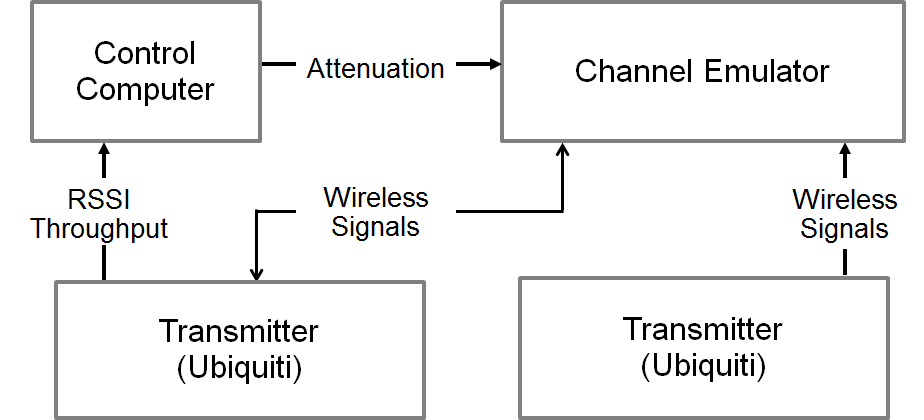
\includegraphics[width=65mm]{figures/emulator2}
%\vspace{-0.1in}
\caption{Experimental setup for channel emulator.}
\label{fig:in-door experiment}
\vspace{-0.1in}
\end{figure}

%\subsection{Signal Level Context-aware information}
\subsection{Experimental Design for In-field Data Collection}
\label{subsec:insitu}
We now describe the in-field experimental design to obtain a data set for
evaluating our multiband algorithms. Two Gateworks boards, each containing
the aforementioned four radios, are installed on two cars.  One node is always
the receiver and at a fixed location. The other node is always the 
transmitter and travels 
around the block of a public park as shown in Figure~\ref{fig:infield}.
One loop of the route will be used as a unit of training in the next section.

\begin{figure} [h]
%\vspace{-0.1in}
\centering
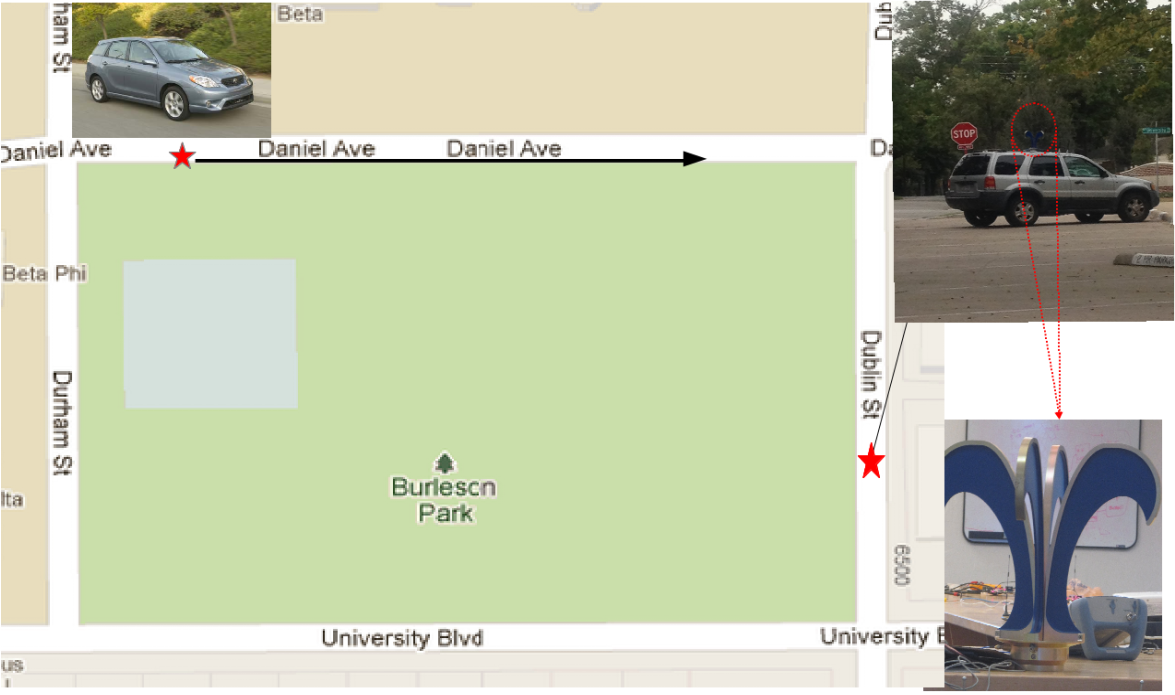
\includegraphics[width=75mm]{figures/infield}
\vspace{-0.1in}
\caption{In-field Experimental Setup.}
\label{fig:infield}
\vspace{-0.1in}
\end{figure}

During each loop, the transmitter sends a fully-backlogged UDP flow
using {\it iperf} on each of the four radios simultaneously.  To
focus on band selection and ensure the greatest range, we disable autorate and use a fixed data rate
of 6 Mbps. The receiver continually performs a {\it tcpdump} of all
received 802.11 packets~\cite{jacobson1989tcpdump}. Additionally, a
QH 400 Quad Ridge Horn Antenna (shown in Figure~\ref{fig:infield}) is 
connected to a Rhode \& Schwarz FSH8 mobile spectrum analyzer at the 
receiver to monitor spectral activity. Then, based on the 
time stamps, we remove 802.11 packets from the spectral trace 
so that only non-802.11 interference will contribute to $P_N^i$.

\begin{figure} 
%\vspace{-0.1in}
\centering
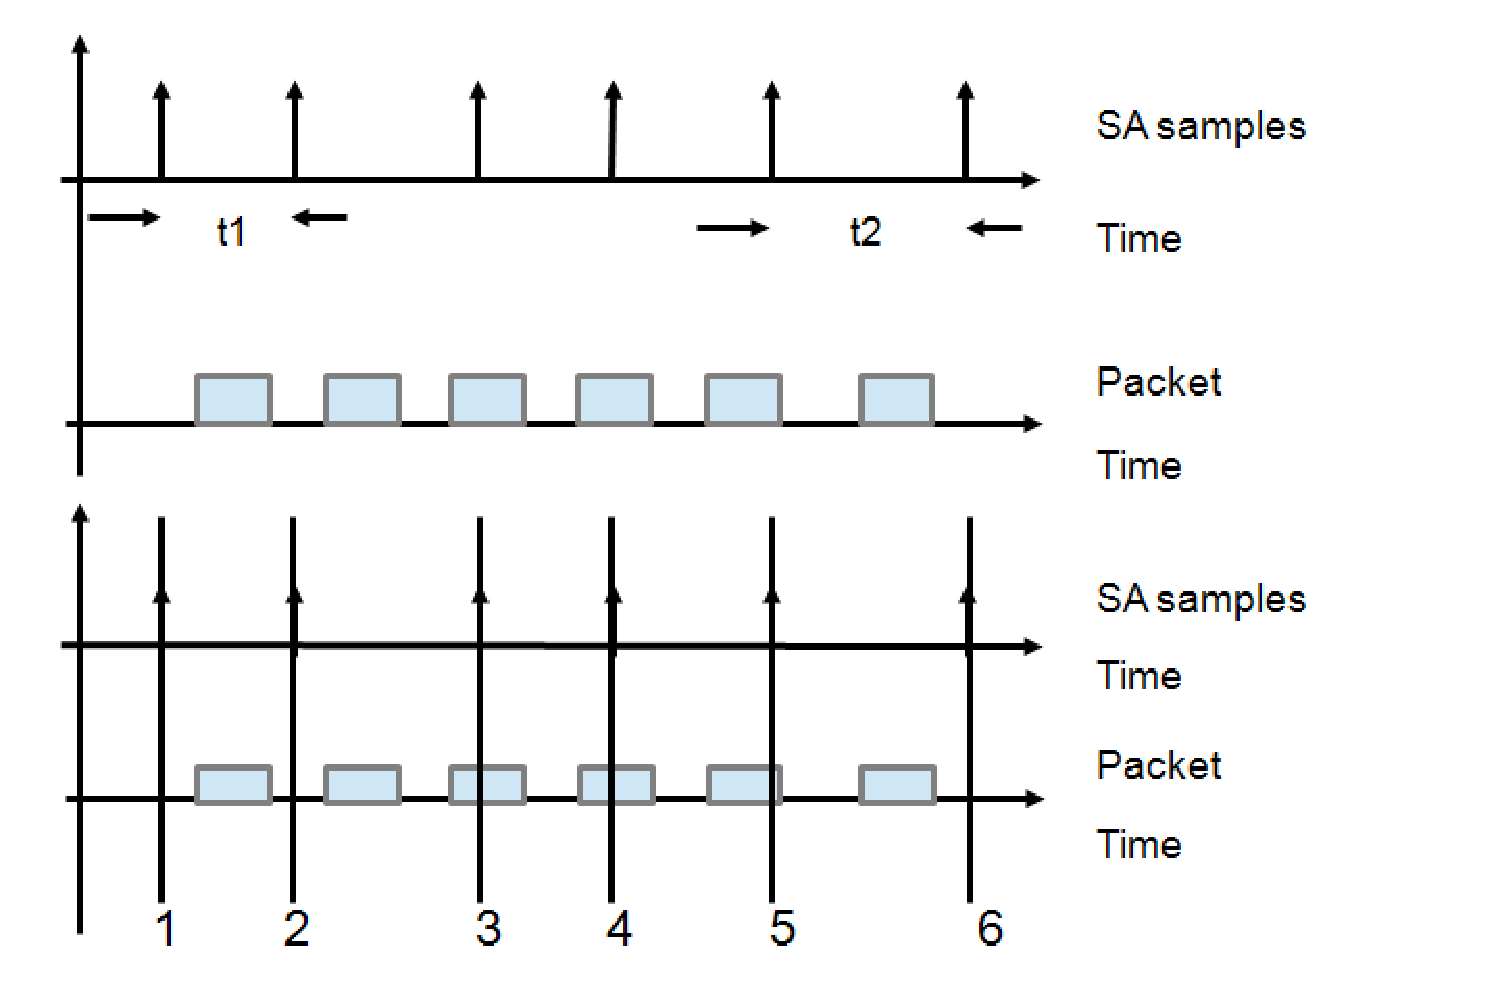
\includegraphics[width=75mm]{figures/sa_process}
\vspace{-0.1in}
\caption{Spectrum Analyzer Data Processing.}
\label{fig:sa_process}
\vspace{0.1in}
\end{figure}

Figure~\ref{fig:sa_process} shows how we obtain the
non-802.11 interference, $P_N^i$. We expunge the spectrum analyzer
(SA) samples which overlap in time with the dumped 802.11 packets,
such as packets 3, 4, and 5. Then, the reported interference value
will not contain the received power from 802.11 packets, which have
already been considered via the busy time, $B$.

The in-field data is processed offline where data from all instruments
involved is synchronized based on the GPS time stamps. 
As discussed in Section~\ref{subsec:ichannel}, the throughput of each radio
is normalized based upon emulator experiments to account for any
manufacturing differences.

